


\section{Time graph of the variations of a variable measured at different locations}
\label{sec-1}





    
    
  
  
    
  


The first attempt to display this multivariate time series makes
use of the \texttt{xyplot.zoo} method. The objective of this graphic is
to display the behaviour of the collection as a whole: the series
are superposed in the same panel (\texttt{superpose=TRUE}) without legend
(\texttt{auto.key=TRUE}), using thin lines (\texttt{lwd=0.3}) and partial
transparency (\texttt{alpha=0.3}). Transparency softens overplotting
problems and reveals density clusters since regions with more
overlapping lines are darker. The figure \ref{fig:navarraNaive}
displays the variations around the time average (\texttt{avRad}).

\index{zoo@\texttt{zoo}} 
\index{xyplot.zoo@\texttt{xyplot.zoo}}

\lstset{language=R}
\begin{lstlisting}
avRad <- zoo(rowMeans(navarra, na.rm=1), index(navarra))
pNavarra <- xyplot(navarra - avRad, superpose=TRUE, auto.key=FALSE,
                   lwd=0.3, alpha=0.2, col='black') 
pNavarra
\end{lstlisting}

\begin{figure}[htb]
\centering
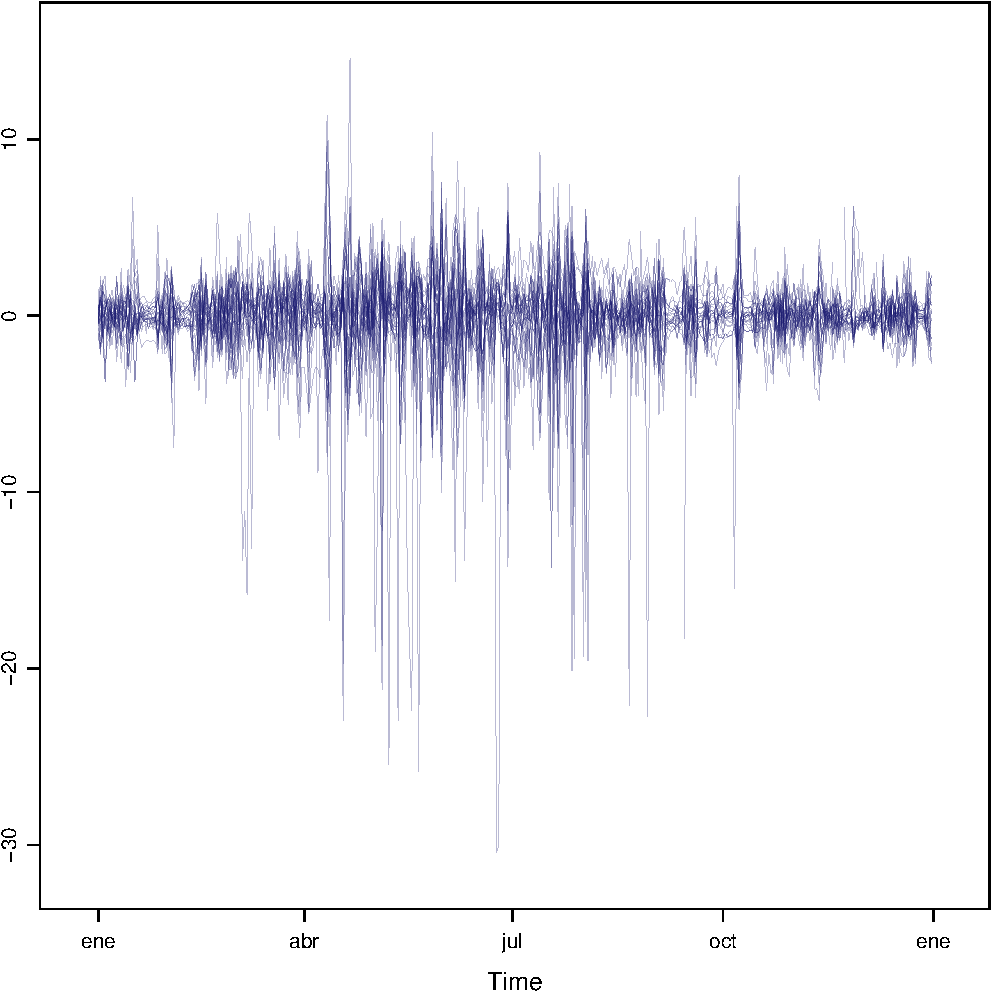
\includegraphics[width=.9\linewidth]{figs/navarra.pdf}
\caption{\label{fig:navarraNaive}Time plot of the variations around time average of solar radiation measurements from the meteorological stations of Navarra.}
\end{figure}

This result can be improved with two different tools: the horizon
graph with \texttt{horizonplot} and dynamic labelling with the \texttt{gridSVG}
package.
\subsection{The horizon graph}
\label{sec-1-1}


The horizon graph\index{Horizon graph} is useful to examine how a
large number of series changes through time, and to do so in a way
that allows both comparisons between the individual time series and
and independent analysis of each series. Moreover,
extraordinary behaviours and predominant patterns are easily
distinguished \cite{Few2008}.

This graph displays several stacked series collapsing the y-axis
to free vertical space:
\begin{itemize}
\item Positive and negative values share the same vertical
  space. Negative values are inverted and placed above the
  reference line. Sign is encoded using different hues (positive
  values in blue and negative values in red).
\item Differences in magnitude are displayed as differences in color
  intensity (darker colors for greater differences).
\item The color bands share the same baseline and are superposed with
  darker bands in front of the ligther ones.
\end{itemize}

Since the panels share the same design structure, once this
technique is understood, it is easy to establish comparisons or
spot extraordinary events.  This method is what Tufte described as
small multiples\index{Small multiples} \cite{Tufte1990}.

Figure \ref{fig:navarraHorizonplot} displays the variations of
solar radiation around the time average with an horizon graph
using a row for each time series.
\index{Packages!latticeExtra@\texttt{latticeExtra}}
\index{horizonplot@\texttt{horizonplot}}

\lstset{language=R}
\begin{lstlisting}
library(latticeExtra)

horizonplot(navarra-avRad, layout=c(1, ncol(navarra)),
            origin=0, colorkey=TRUE)
\end{lstlisting}

\begin{figure}[htb]
\centering
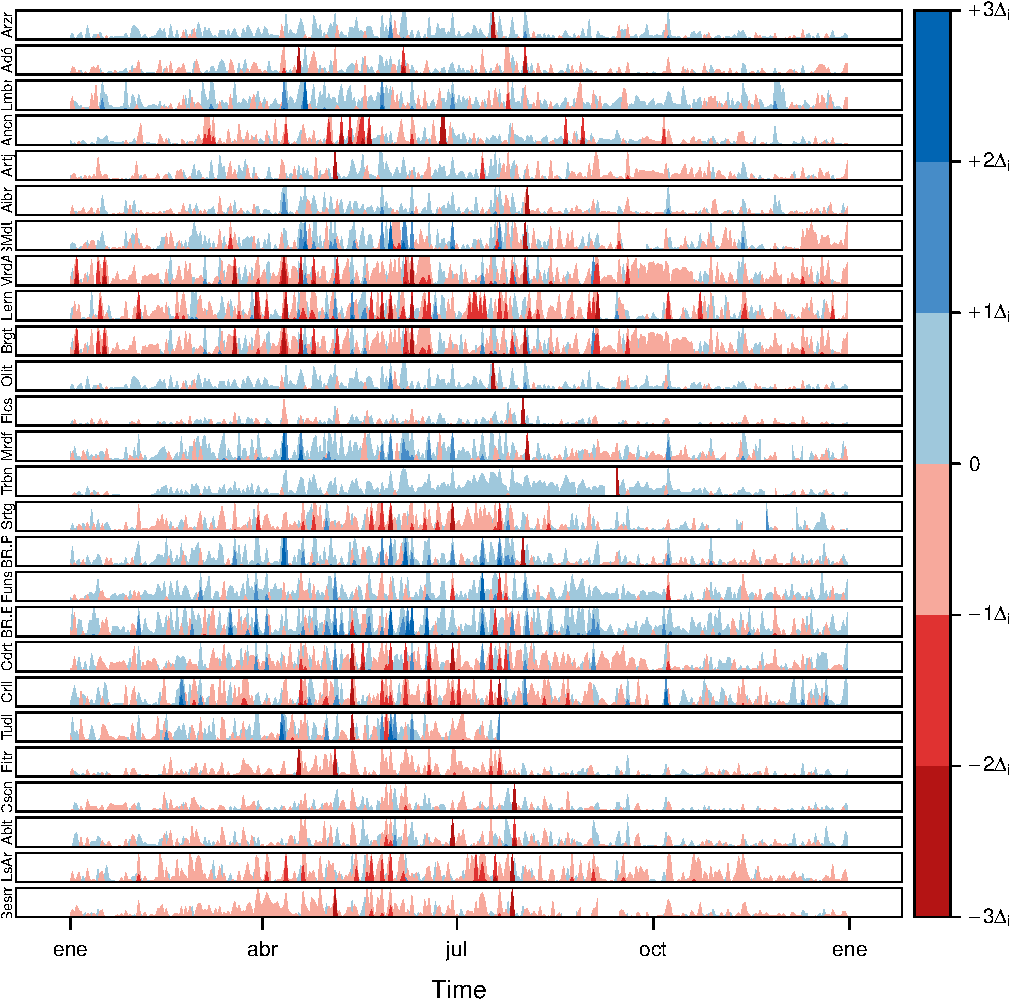
\includegraphics[width=.9\linewidth]{figs/navarraHorizonplot.pdf}
\caption{\label{fig:navarraHorizonplot}Horizonplot of variations around time average of solar radiation measurements from the meteorological stations of Navarra.}
\end{figure}
\subsection{Interaction with \texttt{gridSVG}}
\label{sec-1-2}


The \texttt{gridSVG} package provides functions to convert \texttt{grid}-
based \texttt{R} graphics to an SVG format. It provides several functions
to add dynamic and interactive capabilities to \texttt{R} graphics. In
this section we will use \texttt{grid.script}, a function to add
JavaScript code to a plot.

The first step is to specify which component of the scene
will run the JavaScript code. The \texttt{grid.ls} function  returns a
listing of the names of grobs or viewports included in the graphic
output: only the lines will be connected with the JavaScript
code. 

\index{Packages!gridSVG@\texttt{gridSVG}}
\index{grid.ls@\texttt{grid.ls}}

\lstset{language=R}
\begin{lstlisting}
library(gridSVG)
## grobs in the graphical output
pNavarra
grobs <- grid.ls(print=FALSE)
## only interested in some of them
nms <- grobs$name[grobs$type == "grobListing"]
idxNames <- grep('lines', nms)
IDs <- nms[idxNames]
\end{lstlisting}


The second step is to modify each \texttt{grob} (graphical object) to add
attributes that specify when it will call JavaScript code. For
each line identified with the elements of the \texttt{IDs} vector and
associated to a meteorological station, the \texttt{navarra} object is
accessed to extract the annual mean value of the daily radiation
and the abbreviated name of the corresponding station.  The
\texttt{grid.garnish} function adds attributes to the \texttt{grob} of each line
so that when the mouse moves over a grob a tooltip is displayed to
show the information defined by \texttt{info} and the line is highlighted
and colored in red, and to hide the tooltip and to set the default
parameters of the line when the mouse hovers out of the \texttt{grob}.

\index{grid.garnish@\texttt{grid.garnish}}

\lstset{language=R}
\begin{lstlisting}
for (id in unique(IDs)){
  ## extract information from the data
  ## according to the ID value
  i <- strsplit(id, '\\.')
  i <- sapply(i, function(x)as.numeric(x[5]))

  ## Information to be attached to each line: annual mean of daily
  ## radiation and abbreviated name of the station
  dat <- round(mean(navarra[,i], na.rm=TRUE), 2)
  info <- paste(names(navarra)[i], paste(dat, collapse=','),
                sep=':')
  ## attach SVG attributes
  grid.garnish(id,
               onmouseover=paste("showTooltip(evt,'", info, "')"),
               onmouseout="hideTooltip(evt)")
}
\end{lstlisting}


Finally, \texttt{grid.script} adds a script file that contains the
JavaScript code to draw the tooltips and \texttt{gridToSVG} exports
the whole scene to SVG. 

\index{grid.script@\texttt{grid.script}}
\index{gridToSVG@\texttt{gridToSVG}}
\index{Javascript}

\lstset{language=R}
\begin{lstlisting}
grid.script(filename="tooltip.js")
gridToSVG('figs/navarraRadiation.svg')
\end{lstlisting}


A snapshot of the result, as viewed in a browser with a line
highlighted, is shown in Figure \ref{fig:navarraSVG}.

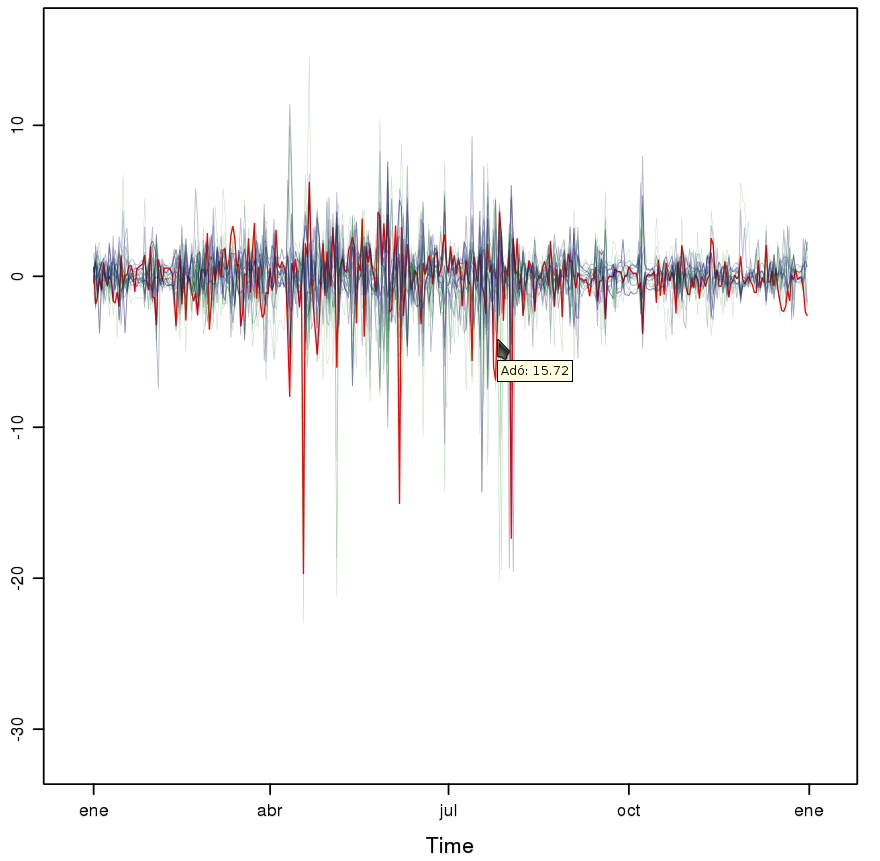
\includegraphics{figs/navarraSVG_captura.png}
